\documentclass{standalone}
\usepackage{tikz}
\usepackage{color}
\usetikzlibrary{positioning, shapes, arrows.meta, calc, decorations.pathreplacing}

\definecolor{myblue}{RGB}{82,126,171}
\definecolor{myred}{RGB}{168, 50, 50}

\tikzset{
  square/.style={draw,outer sep=5,inner sep=3,minimum size=10,line width=0, 
    very thick, draw=myblue, top color=white,bottom color=white},
  noborder/.style={draw,outer sep=0,inner sep=0,minimum size=20,line width=1, 
    draw=none, scale=1, anchor=west},
  blue/.style={draw,outer sep=35,inner sep=3,minimum size=20, line width=1, 
    very thick, draw=none, top color=myblue, bottom color=myblue, scale=1.25},
   noborderr/.style={draw,outer sep=0,inner sep=0,minimum size=20,line width=1, 
    draw=none, scale=1, anchor=west}
}

\begin{document}

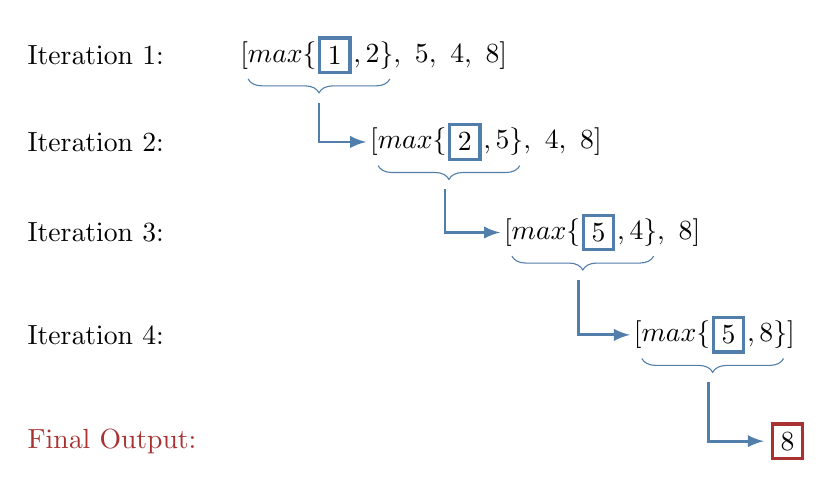
\begin{tikzpicture}[>={Latex[width=2mm,length=2mm]}]



\draw[decorate,color=myblue,decoration={brace,amplitude=5pt}] (0.35,1.4) -- (-1.45,1.4);
\draw[-latex,line width=1 pt,color=myblue] (-0.55,1.1) |- (0.05,0.6);

\node [noborderr] at (-1.55,1.7) {$[max\{~~~~,2\}, ~5, ~4, ~8]$};
\node [square] at (-0.35,1.7) {$1$};


\draw[decorate,color=myblue,decoration={brace,amplitude=5pt}] (2,0.3) -- (0.2,0.3);
\draw[-latex,line width=1 pt, color=myblue] (1.05,0) |- (1.75,-0.55);

\node [noborderr] at (0.1,0.6) {$[max\{~~~~,5\},  ~4, ~8]$};
\node [square] at (1.3,0.6) {$2$};


\draw[decorate,color=myblue,decoration={brace,amplitude=5pt}] (3.7,-0.85) -- (1.9,-0.85);
\draw[-latex,line width=1 pt,color=myblue] (2.75,-1.15) |- (3.4,-1.85);

\node [noborderr] at (1.8,-0.55) {$[max\{~~~~,4\},  ~8]$};
\node [square] at (3,-0.55) {$5$};


\draw[decorate,color=myblue,decoration={brace,amplitude=5pt}] (5.35,-2.15) -- (3.55,-2.15);
\draw[-latex, line width=1 pt, color=myblue] (4.4,-2.45) |- (5.1,-3.2);

\node [noborderr] at (3.45,-1.85) {$[max\{~~~~,8\}]$};
\node [square] at (4.65,-1.85) {$5$};
\node [square,draw=myred] at (5.4,-3.2) {$8$};

\node [noborderr] at (-4.25,1.7) {Iteration 1:};
\node [noborderr] at (-4.25,0.6) {Iteration 2:};
\node [noborderr] at (-4.25,-0.55) {Iteration 3:};
\node [noborderr] at (-4.25,-1.85) {Iteration 4:};
\node [noborderr, color=myred] at (-4.25,-3.2) {Final Output:};


\end{tikzpicture}

\end{document}
